\documentclass{../notatki}
\usepackage{physics}

\title{Wstęp do Fizyki Kwantowej}

\begin{document}

\section{Wstęp}

Przydatne wzory w jednym miejscu:
\begin{itemize}
  \item Pęd ciałą o masie $m$ i prędkości $v$:
    $$
    p = mv
    $$
  \item Energia ciała o masie $m$ i pędzie $p$: $$
    E^2 =c^2p^2 + m^2c^4
    $$
  \item Stała plancka i jej \textbf{evil twin} $$
    h = 2 \pi \hbar
    $$
  \item Prędkość fali $$
    v = \lambda \nu
    $$
\end{itemize}

\subsection{Algebra}

\textit{Z jakiegoś powodu dużą częścią zajęć była algebra, bo fizycy nie mieli
  dedykowanego przedmiotu, więc tu przypomnienie bo pewno algebra będzie sporą
częścią kolowkium \texttt{<3}}.

\subsubsection{Macierze}

$$
A_{ij} = A^T_{ji}
$$

$$
\overline{a + b\textit{i}} = a - b\textit{i}
$$

$$
A^\dag = \overline{A}^T
$$

\begin{itemize}
  \item Symetryczna $A^T = A$
  \item Ortogonalna $A^T \cdot A = A \cdot A^T = I$
  \item Hermitowska $A^\dag = A$
  \item Normalna $A^\dag \cdot A = A \cdot A^\dag$
  \item Unitarna $A^\dag \cdot A = A \cdot A^\dag = I$
  \item Osobliwa $\det A = 0$
\end{itemize}

\subsubsection{Wartości i wektory własne}

$$
\det(A - \lambda I) = 0
$$

$$
(A - \lambda_i I)v_i = 0
$$

\subsubsection{Notacja Diraca}

Wektor $v$, nazwany $a$ w przestrzeni $V$ (domyślnie $\mathbb{C}^n$)
można zapisać jako:
$$
\ket{a} = v = (v_1, v_2, \ldots, v_n)
$$

$$
\bra{a} = \ket{a}^\dagger
$$

$$
\braket{a}{b} = \bra{a} \cdot \ket{b} = \sum_{i} \overline{a_i} b_i
$$

$$
\ketbra{a}{b} = \ket{b} \times \bra{a}
$$

\subsubsection{Rozkład spektralny}

Dla każdej macierzy normalnej $A$ istnieje jej rozkład spektralny, czyli:
$$
A = \sum_{i} \lambda_i P_i = \sum_{i} \lambda_i \ketbra{i}{i}
$$

\subsubsection{Diagonalizacja}

$$
A = UDU^{-1}
$$
Dla macierzy normalnej $U^{-1} = U^\dag$. $U$ to macierz złożona z
wektorów własnych $A$. $D$ to macierz diagonalna, gdzie wszystkie wartości
występujące na przekątnej to wartości własne $A$, lub inaczej, jest to macierz
zapisana w bazie swoich wektorów własnych.

$$
f(A) = U^\dag
\begin{bmatrix}
  f(\lambda_1) & 0 & \cdots & 0 \\
  0 & f(\lambda_2) & \cdots & 0 \\
  \vdots & \vdots & \ddots & \vdots \\
  0 & 0 & \cdots & f(\lambda_n)
\end{bmatrix} U
$$

Magicznym aspektem macierzy zdiagonalizowanych, lub szerzej, tych zapisanych
w bazie swoich wektorów własnych, jest to, że na ich diagonali są ich wartości
własne.

\subsubsection{Operacje}

$$
\trace(A) = \sum_{i} \lambda_i = \sum_{i} A_{ii}
$$
$$
\det(A_{2 \times 2}) = A_{11}A_{22} - A_{12}A_{21}
$$
$$
[A, B] = AB - BA
$$

\section{Eksperyment Younga - dwu-szczelinowy}

W eksperymencie mierzymy zachowanie elektronów względem
dwóch dziur i czujnika ruchomego na wzdłuż osi $x$. Mierzymy prawdopodobieństwo,
tego, że czujnik odbierze elektron, jako $P_{12}(x)$. Równocześnie rozróżniamy
$P_1(x)$ oraz $P_2(x)$; prawdopodobieństwa, tego, że czujnik odbierze
elektron przy jednej z dziur zasłoniętej. Diagram ilustrujący eksperyment
znajduje się w \cref{fig:young}.
\begin{figure}[H]
  \centering
  \begin{tikzpicture}
    \node[draw] (source) at (-4,2) {źródło};

    \draw (0,0) -- (0, 1.8);
    \draw (0, 2) -- (0, 2.3);
    \draw (0, 2.5) -- (0,4);

    \draw[thick] (2,0) -- (2,4) node[above] {$x$};

    \draw[->] (source.east) -- (0, 2.4);
    \draw[->] (source.east) -- (0, 1.9);

  \end{tikzpicture}
  \caption{Ilustracja eksperymentu}
  \label{fig:young}
\end{figure}

\subsection{Cząstkowa interpretacja}

Jeśli elektron zachowałby się jako cząstka, to spodziewalibyśmy się, że
$P_{12}(x) = P_1(x) + P_2(x)$. Wnioskiem takiej obserwacji byłoby, że
cząstki elektronów nie mają na siebie wpływu; nie zachodzi interferencja.
Co więcej, elektron zawsze przechodzi jedną dziurą.

\subsection{Falowa interpretacja}

Jeśli elektron zachowałby się jako fala, to spodziewalibyśmy się
przeciwnego wyniku. Fale nie nakładają się na siebie tak czysto.
Zachodziłaby interferencja; fale w zależności od fazy albo by się na siebie
nakładały, albo niwelowały. Co więcej ze wzlędu na działanie fal, elektron
by przechodził przez obydwie dziury jednocześnie.
$P_{12}(x) = |\phi_1(x) + \phi_2(x)|^2$,
$P_1 = |\phi_1(x)|^2$, \dots.

\subsection{Wynik}

Eksperyment pokazuje, że mimo tego, że detektor odbiera elektrony
w dyskretnych grupach, to $P_{12}$ zachowuje się jakby elektrony były falami.
Zatem elektron zachowuje się "trochę jak cząstka trochę jak fala".

Obserwowanie elektronów, które przechodzą przez szczeliny, powoduje,
że przestają zachowywać się jak fale, a zaczynają zachowywać się jak cząstki.
Znika inteferencja, bo wiemy, że elektron przechodzi przez jedną z
dziur, a nie przez obydwie.

Na podstawie tego eksperymentu, opracowano zasadę niepewności Heisenberga.
W ramach eksperymentu, oznacza ona, że nie da się zaprojektować detektora
elektronów, który nie wpływa na elektrony. Detektor, czy to pozycji czy pędu,
ma pewną dokładność i pomiar tej dokładności wpływa na mierzoną cząstkę.
Zasada niepewności nie wpływa na życie na naszej skali, ponieważ długości fali
obiektów w naszej skali są bardzo małe, oraz te obiekty są obserwowane ciągle,
więc nie ma możliwości, żeby zachowywały się jak fale.

\subsection{Słabe źródło światła}

Z słabym źródłem światła, możemy się spodziewać pojedynczych fotonów, które
trafiają w losowe punkty na ekranie. Po dłuższym czasie, możemy
zauważyć, że rozkład tych punktów przypomina rozkład interferencyjny,
który obserwujemy w przypadku silnego źródła światła.
To dowodzi istnienia fotonów.

\subsection{Wyprowadzenia}

Ten eksperyment pozwala nam wyprowadzić następujące właściwości
światła o danej długości fali $\lambda$ i częstości $\omega$:

$$
k = \frac{2 \pi}{\lambda}
$$
$$
p = \frac{2\pi\hbar}{\lambda} = \frac{h}{\lambda} = k\hbar
$$
$$
E_f = \hbar \omega = pc = h \nu
$$
Zatem też: $m_f = 0$, $v_f = c$.

\subsection{Światło}

\noindent \textit{Światło o danym $\lambda$ i $\omega$ składa się z
dyskretnych cząstek, których dystrybucja jest dana przez interferencję fali}.
Nie jest falą, ale działa jak fala. Charakterystyka fali określa
prawdopodobieństo, tego że foton padnie w danym miejscu.
Co więcej, foton wie czy szczelina jest otwarta w eksperymencie
dwu-szczelinowym, co ma sens tylko jeśli jest falą.
Należy też wspomnieć, że foton nie może się zatrzymać. Jako, że nie ma masy,
to pęd i jego energia są zależne od jego prędkości. Gdyby się
zatrzymał, to jego energia i pęd byłyby równe zero, co jest
niemożliwe z zachowania energii.

\subsection{Fala de Broglie}

Jest to generalizacja koncepcji światła wychodzącej z eksperymentu Younga.
Każda fala, która na skali makroskopicznej zachowuje się jak fala, lecz tak
naprawdę jest masą dyskretnych cząstek jest falą de Broglie, lub falą materii.

$$
\lambda = \frac{h}{p}
$$

Elektron jak i foton są falami de Broglie, ale foton jest falą de
Broglie o masie zerowej.

\section{Zasada niepewności}

$$
\Delta x \Delta p \geq \frac{\hbar}{2}
$$
gdzie, na przykład, $\Delta x = \sigma(x)$. Istotna jest jednak obserwacja, że
dla $\Delta x \rightarrow 0$, $\Delta p \rightarrow \infty$, i na odwrót.

\section{Efekt Fotoelektryczny}

W wyniku promieniowania fotonami, elektrony atomów pierwiastka są
wyrzucane z atomu. Efekt ten jest wykorzystywany w praktyce w
napędzaniu fotodiod i fotokomórek.

Elektrony w metalu znajdują się w studni potencjału, głębokości $W$,
odpowiadającej pracy wyjścia.
Foton padając na materiał powoduje wyrzucenie elektronu naładowanego
$U$ z energią kinetyczną $E_{k \text{max}}$. $U$ nazywamy potencjałem
hamującym. W wyniku tego procesu
utracona zostaje energia w postaci pracy wyjścia $W$:
$$
E_{k \text{max}} = E_f - W = eU
$$
Częstością progową nazywamy najniższą częstość $\omega_0$, dla której
$E_{k \text{max}} = 0$.

Einstein w 1905 sugerował, istnienie fotonów, jako cząstek światła,
aby wyjaśnić efekt fotoelektryczny. Rzeczywiście, w formaliźmie
powyżej ma to sens.

\section{Zjawisko Comptona}

W zjawisku Comptona foton padający na elektron zmienia kierunek i
częstość. Efekt ten jest wykorzystywany w praktyce w analizie struktury
atomów i molekuł. Ilustracja zjawiska znajduje się w \cref{fig:compton}.
\begin{figure}[H]
  \centering
  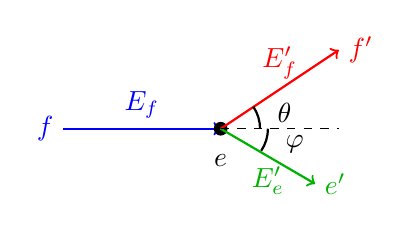
\begin{tikzpicture}
    \draw[->,thick,blue] (-2,0) -- (0,0) node[midway,above] {$E_f$};
    \draw[blue] (-2,0) node[left] {$f$};

    \draw[fill=black] (0,0) circle (0.08);
    \draw (0,-0.2) node[below] {$e$};

    \draw[->,thick,red] (0,0) -- (1.5,1) node[midway,above] {$E_f'$};
    \draw[red] (1.5,1) node[right] {$f'$};

    \draw[->,thick,green!70!black] (0,0) -- (1.2,-0.7)
    node[midway,below] {$E_e'$};
    \draw[green!70!black] (1.2,-0.7) node[right] {$e'$};

    \draw[thick] (0.5,0) arc (0:34:0.5);
    \draw (0.6,0.2) node[right] {$\theta$};

    \draw[thick] (0.6,0) arc (0:-34:0.5);
    \draw (0.7,-0.2) node[right] {$\varphi$};

    \draw[dashed] (0,0) -- (1.5,0);
  \end{tikzpicture}
  \caption{Ilustracja zjawiska Comptona. Foton $f$ ma długość fali $\lambda$.}
  \label{fig:compton}
\end{figure}

W zjawisku zachowanny jest pęd oraz energia, co wraz z równaniem Comptona:
$$
(\lambda' - \lambda) \frac{m_ec}{h} = 1 - \cos\theta
$$
Pozwala nam w istocie wyprowadzić wszystkie niewadome w zjawisku.

$$
p_f + p_e = p_f' + p_e' \Rightarrow
\begin{cases}
  \frac{h}{\lambda} = \frac{h}{\lambda'}\cos\theta + p_e'\cos\varphi \\
  0 = \frac{h}{\lambda'}\sin\theta + p_e'\sin\varphi
\end{cases}
$$

$$
E_f + E_e = E_f' + E_e' \Rightarrow \frac{hc}{\lambda} + m_ec^2 =
\frac{hc}{\lambda'} + E_e'
$$

Efekt comptona, opisany w 1927 roku, jest dowodem na istnienie fotonu.

\section{Model Bohra}

Do opracowania modelu atomu Bohra, przyczynił się eksperyment J. Balmera. W tym
eksperymencie światło przechodzące przez gaz pewnego pierwiastka,
rozszczepia się na tylko konkretne kolory. To eksperymentalnie sugeruje, że
atom może emitować tylko dyskretne poziomy energii.

W modelu atomu Bohra, elektron porusza się wokół jądra wokół jednej z
dyskretnych
orbit. To też oznacza, że energia elektronu jest dyskretna lub zkwantowana.
Diagram modelu można znaleźć w \cref{fig:bohr}.
\begin{figure}[H]
  \centering
  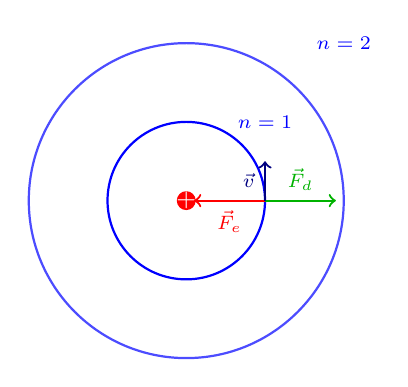
\begin{tikzpicture}
    \fill[red] (0,0) circle (0.12) node[white] {\small +};

    \draw[thick,blue] (0,0) circle (1);
    \draw[thick,blue,opacity=0.7] (0,0) circle (2);

    \node[blue] at (1,1) {\scriptsize $n=1$};
    \node[blue] at (2,2) {\scriptsize $n=2$};

    \draw[->,thick,green!70!black] (1,0) -- (1.9,0)
    node[midway,above] {\scriptsize $\vec{F}_d$};

    \draw[->,thick,red] (1,0) -- (0.1,0)
    node[midway,below] {\scriptsize $\vec{F}_e$};

    \draw[->,thick,blue!50!black] (1,0) -- (1,0.5)
    node[midway,left] {\scriptsize $\vec{v}$};

  \end{tikzpicture}
  \caption{Model Bohra atomu}
  \label{fig:bohr}
\end{figure}

Elektron na orbicie utrzymuje się w wyniku siły elektrostatycznej między
elektronem a jądrem.
$$
\frac{mv^2}{r} = k \frac{e^2}{r^2}
$$
$$
L = mvr = n\hbar
$$
Dla dowolnego ciała na orbicie:
$$
v = \frac{2\pi r}{T}
$$
gdzie $T$ jest czasem okresu orbity. Energie potencjalną można wyznaczyć z
pola elektrycznego.
$$
E_p = 2E_k = k\frac{e^2}{r}
$$
$$
E_k = \frac{1}{2}mv^2
$$

\subsection{Nieskończenie głęboka studnia potencjału}

Istnieje studnia potencjału. W zakresie $x \in (0, L)$ cząstka może się poruszać
swobodnie, potencjał jest zerowy. Poza tym obszarem potencjał jest
nieskończenie duży. długość studni ($L$) musi być równa całkowitej
wielokrotności połowy długości fali:
$$
L = n\frac{\lambda}{2}
$$
Trzeba też wykorzystać własności fali de Broglie
($\lambda=\frac{h}{p}$) aby uzyskać:
$$
p_n = \frac{nh}{2L}
$$

Postulat Bohra:
$$
\oint pdq = nh
$$

\subsection{Ciało doskonale czarne}

Ciało doskonale czarne, to koncept fizyczny, w którym rozważamy zachowanie się
energii, temperatury i promieniowana w doskonale czarnej wnęce. Założenie jest
takie, że ciało ma nie dopuścić do powrotnej emisji promieniowania.

W ciele doskonale czarnym zakłada się, że liczba modów oscylacyjnych jest dana
wzorem:
$$
N(\nu)d\nu = \frac{8\pi\nu^2}{c^3}d\nu
$$
Wynika to z $\nu = \frac{c}{\lambda}$ oraz $\lambda = \frac{2\pi}{k}$.
Gęstość energii na jednostkę częsości wyraża się:
$$
u(\nu, T) = N(\nu)\langle E \rangle
$$

\subsubsection{Katastrofa w ultrafiolecie}

W klasycznej teorii z zasady ekwipartycji energii wynika, że średnia
energia przypadająca na jeden stopień swobody układu oscylacyjnego jest równa:
$$
\langle E \rangle = k_BT
$$
Podstawienie $\langle E \rangle = k_BT$ do $u(\nu, T)$ daje nam wzór
Rayleigha-Jeansa na gęstość energii na jednostkę częstośći. Ten wzór jest
o tyle słaby, że całka po całym zakresie $\nu$ daje nam nieskończoną energię,
co jest nonsensem. Ten fenomen został nazwany katastrofą w ultrafiolecie.

\subsubsection{Wzór Plancka}

Planck rozwiązał problem z wzorem Rayleigha-Jeansa, wprowadzając inną
definicję $\langle E \rangle$. Podstawowym założeniem Plancka jest, że energia
pojedynczego oscylatora jest zkwantowana.
$$
E_n = nh\nu
$$
$$
\langle E \rangle = \frac{h\nu}{e^{\frac{h\nu}{k_BT}} - 1}
$$

\subsection{Efekt Einsteina de Haasa}

Zakładano, że magnetyzm się bierze, z ruchu elektronów na orbicie atomu
Bohra. Zgodnie z tym modelem, prąd na pierwszej orbicie powinien wynosić:
$$
I = \frac{e}{T} = \frac{ne\hbar}{2\pi r^2m}
$$
Magnetyczny moment dipolowy $\mu$, wynosi zatem:
$$
\vec{\mu} = I \cdot \vec{S} = I \cdot \pi r^2 = \frac{-e}{2m} \vec{L}
= \frac{-e}{2m} \hbar
$$
Ta wartość nie zgadzała się z wynikami eksperymentów, ponieważ nie uwzględniała
spinu elektronów jako większej składowej magnetyzmu. Zatem eksperymentalnie:
$$
\frac{\mu}{L} = g(\frac{-e}{2m})
$$

\subsection{Eksperyment Sterna-Gerlacha}

Srebro $\texttt{Ag}_{47}$ ma tylko jeden wolny elektron. W wyniku ogrzewania
srebra, odłącza się ten pojedynczy elektron. Jeśli na drodze elektronu
znajduje się pole magnetyczne, to elektron odbija się w pewnym kierunku.
W wyniku tego eksperymentu można wywnioskować, że elektron ma spin.
$$
\vec{\mu_s} = g\frac{-e}{2m} \vec{S}
$$

Wykonanie wielokrotne eksperymentu Sterna-Gerlacha(SG), pozwala nam wyprowadzić
kilka podstawowych zasad fizyki kwantowej.
\begin{figure}[h]
  \centering
  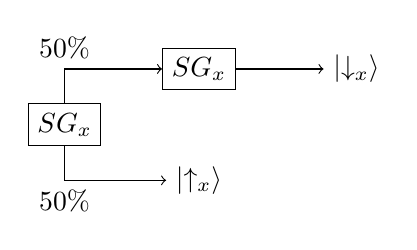
\begin{tikzpicture}
    \node[draw] (sg11) at (0,0) {$SG_x$};
    \node[draw, above right of=sg11, xshift=1cm] (sg12) {$SG_x$};
    \node[below right of=sg11, xshift=1cm] (sg13) {$\ket{\uparrow_x}$};
    \node[right of=sg12, xshift=1cm] (sg14) {$\ket{\downarrow_x}$};

    \draw[->] (sg11) |- node[above] {50\%} (sg12);
    \draw[->] (sg11) |- node[below] {50\%} (sg13);
    \draw[->] (sg12) -- (sg14);
  \end{tikzpicture}
  \caption{Sekwencyjny eksperyment Sterna-Gerlacha 1}
  \label{fig:sg1}
\end{figure}
Diagram \cref{fig:sg1} ilustruje jak elektron w fizyce kwantowej ma konkretny
stan spinu w danej osi.

Powtórzenie eksperymentu, lecz tym razem za drugim podejściem mierzenie
wobec innej osi, daje nam zupelnie inny wynik. Ilustracja tego
procesu znajduje się w \cref{fig:sg2}.
\begin{figure}[h]
  \centering
  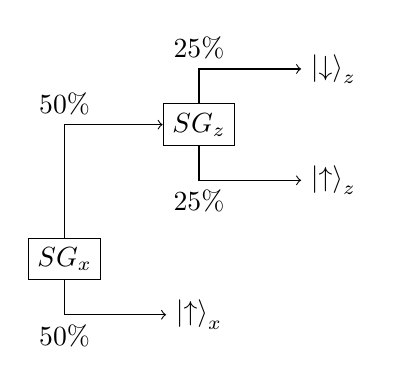
\begin{tikzpicture}
    \node[draw] (sg11) at (0,0) {$SG_x$};
    \node[draw, above right of=sg11, xshift=1cm, yshift=1cm] (sg12) {$SG_z$};
    \node[below right of=sg11, xshift=1cm] (sg13) {$\ket{\uparrow}_x$};
    \node[above right of=sg12, xshift=1cm] (sg14) {$\ket{\downarrow}_z$};
    \node[below right of=sg12, xshift=1cm] (sg15) {$\ket{\uparrow}_z$};

    \draw[->] (sg11) |- node[above] {50\%} (sg12);
    \draw[->] (sg11) |- node[below] {50\%} (sg13);
    \draw[->] (sg12) |- node[above] {25\%} (sg14);
    \draw[->] (sg12) |- node[below] {25\%} (sg15);
  \end{tikzpicture}
  \caption{Sekwencyjny eksperyment Sterna-Gerlacha 2}
  \label{fig:sg2}
\end{figure}
Stany spinów w różnych osiach są niezależne i nie wpływają na siebie, zatem
pomiar w innej osi daje nam kolejny podział na pół elektronów.

Trzykrotne wykonanie eksperymentu SG daje nam najciekawszy wynik. Ilustracja
tego procesu znajduje się w \cref{fig:sg3}.
\begin{figure}[h]
  \centering
  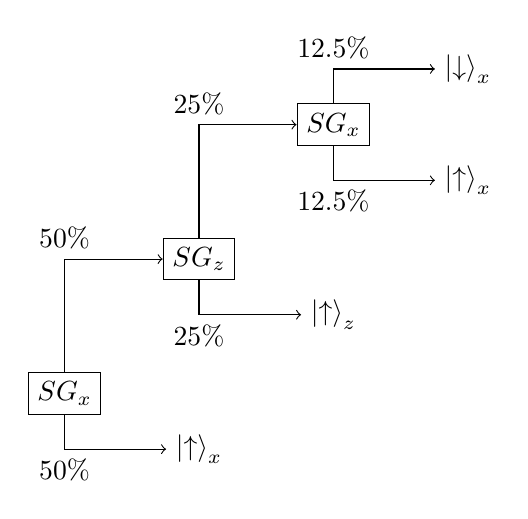
\begin{tikzpicture}
    \node[draw] (sg11) at (0,0) {$SG_x$};
    \node[draw, above right of=sg11, xshift=1cm, yshift=1cm] (sg12) {$SG_z$};
    \node[below right of=sg11, xshift=1cm] (sg13) {$\ket{\uparrow}_x$};
    \node[draw, above right of=sg12, xshift=1cm, yshift=1cm] (sg14) {$SG_x$};
    \node[below right of=sg12, xshift=1cm] (sg15) {$\ket{\uparrow}_z$};
    \node[above right of=sg14, xshift=1cm] (sg16) {$\ket{\downarrow}_x$};
    \node[below right of=sg14, xshift=1cm] (sg17) {$\ket{\uparrow}_x$};

    \draw[->] (sg11) |- node[above] {50\%} (sg12);
    \draw[->] (sg11) |- node[below] {50\%} (sg13);
    \draw[->] (sg12) |- node[above] {25\%} (sg14);
    \draw[->] (sg12) |- node[below] {25\%} (sg15);
    \draw[->] (sg14) |- node[above] {12.5\%} (sg16);
    \draw[->] (sg14) |- node[below] {12.5\%} (sg17);
  \end{tikzpicture}
  \caption{Sekwencyjny eksperyment Sterna-Gerlacha 3}
  \label{fig:sg3}
\end{figure}
Pomiar spinu w osi Z, usunał nam informację o spinie w osi X. Stan spinu
w osi X stał się nieokreślony, aż do ostatniego pomiaru, który dał nam
znowu kolejny podział elektronów na pół.

\section{Postulaty fizyki kwantowej}

\begin{itemize}
  \item Każdy stan układu kwantowego jest opisany przez wektor w
    przestrzeni Hilberta.
    Iloczyn skalarny takich wektorów $\braket{\psi'}{\psi}$ określa amplitudę
    przejścia z stanu $\ket{\psi}$ do stanu $\ket{\psi'}$.
  \item Wielkością, którą można mierzyć odpowiadają operatory
    Hermitowskie - macierze Hermitowskie.
  \item Możliwymi wartościami pomiaru są wartości własne operatora
    Hermitowskiego.
  \item W wyniku pomiaru wartości własnej operatora, układ przeskakuje do
    odpowiadającego stanu własnego (wektora własnego).
\end{itemize}

\section{Stan cząstki}

Z powyższych sekcji wiemy, że cząstka w mechanice kwantowej nie ma stricte
określonej pozycji ani pędu. Wynika to z zasady niepewności Heisenberga.
W mechanice klasycznej cząstki opisujemy parą $(x, p)$, czym opisujemy w
mechanice kwantowej? Mamy funkcję falową $\psi(x)$, gdzie $P(x) = |\psi(x)|^2$
opisuje prawdopodobieństwo znalezienia cząstki w $x$. Nazywamy to postulatem
Borna, oraz:
$$
P(x) = |\psi(x)|^2 = \psi^*(x)\psi(x)
$$
gdzie $\psi^*(x)$ jest sprzężeniem zespolonym funkcji falowej $\psi(x)$.

Elektron w okolicy atomu $1$ jest opisany przez funkcję falową $\psi_1(x)$.
Prawdopodobieństwo tego, że elektron jest w miejscu $x$ obok atomu $1$ opisuje
analogicznie $P_1(x) = |\psi_1(x)|^2$. Teraz wyobraźmy sobie, że
dodajemy drugi atom $2$ i nie wiemy obok
którego jest elektron. Na podstawie pomiarów możem określić, czy pomiary
odpowiadają $P_1(x)$, czy $P_2(x) = |\psi_2(x)|^2$.

Co jeśli elektron może być między cząstkami, czyli nie zakładamy, że należy
do jednej cząstki? Wtedy mówimy, że elektron jest w stanie $\psi_{1 +
2}(x) = \psi_1(x) + \psi_2(x)$. $P_{1 + 2} = |\psi_{1 + 2}|^2$.

\subsection{Pomiar}

Do momentu pomiaru, elektron w naszym przykładzie \textbf{nie ma
pozycji}. Założenie, że
jest obok jednej cząstki jest jak założenie, że cząstka przeszła przez jeden
otwór w eksperymencie Younga. Prawdopodobieństwo w mechanice
klasycznej i kwantowej działają zupełnie inaczej. W mechanice klasycznej
cząstki mają określony zawczasu stan. Pomiar, wykonany w danym czasie uzyska
zawsze jeden wynik. Identyczny pomiar wykonany w mechanice kwantowej może
uzyskać różne odpowiedzi.

Można to sobie wyobrazić w następujący sposób. W mechanice
klasycznej, prawdopodobieństwo $P(x)$ jest ewaluowane a priori.
Mechanika klasyczna jest deterministyczna i znając $(x, p)$ nie muszę
nawet robić pomiarów. W mechanice kwantowej $P(x)$ jest ewaluowane w czasie
rzeczywistym. Mechanika kwantowa nie jest deterministyczna.

\subsection{Funkcja}

$P(x) = |\psi(x)|^2$ musi być całkowalna po całej powierzchni.
Prawdopodobieństwo musi być skończone w końcu. Są od tej zasady
wyjątki, szczególnie cząstki, których całka rośnie wraz z rozmiarem
wszechświata.

Dla cząstki z określonym pędem $p$ postulujemy, że:
$$
\psi_p(x) = A\exp[\frac{ipx}{\hbar}]
$$
$A$ to czynnik normalizujący, wychodzący z konieczności
$1 = \int_{-\infty}^{\infty} |\psi_x(x)|^x dx$. Dla nieskończonego
wszechświata nie ma to sensu, bo $1 = |A|^2 \cdot \infty$.
Zatem zakładamy skończony wszechświat o obwodzie $L$:
$$
\psi_p(x) = \frac{1}{\sqrt{L}}\exp[\frac{ipx}{\hbar}]
$$

Z zasady niepewności wiemy, że skoro w stanie $\psi_p$ mamy określony pęd, to
nie możemy określić z żadną dokładnością pozycji cząstki. Łatwo to
można udowodnić,
albowiem:
$$
P(x) = |\psi_p(x)|^2 =
\frac{1}{\sqrt{L}}\exp[\frac{ipx}{\hbar}]\frac{1}{\sqrt{L}}\exp[-\frac{ipx}{\hbar}]
= \frac{1}{L}
$$
Prawdopodobieństwo jest jednostajne na całej powierzchi wrzechświata. Zasada
niepewności jest spełniona.

\subsection{Warunek kwantyzacji}

Ponieważ wszechświat jest mniej więcej kołem, to funkcja falowa może
być parametryzowana
przez kąt $\theta$. W takiej postaci:
$$
\psi(\theta) = \psi(\theta + 2\pi)
$$
Nazywamy to warunkiem jednej wartości funkcji falowej.

Rozważmy teraz ten warunek w $\psi_p$.
Po nałożeniu warunku jednej wartości falowej, otrzymujemy:
$$
\psi_p(x) = \psi_p(x + L) = \psi_p(x) \exp[\frac{ipL}{\hbar}]
$$
Zatem $\exp[\frac{ipL}{\hbar}] = 1$. Z własności $\exp$ można wyprowadzić, że:
$$
\frac{pL}{\hbar} = 2\pi n
$$
W ten sposób otrzymujemy warunek kwantyzacji:
$$
p_n = \frac{nh}{L}
$$
$$
\psi(x) = \sum_{p} A(p) \psi_p(x)
$$

\subsection{Obserwacje}

Wyobraźmy sobie, że mamy układ, w którym możemy powiedzieć, że zachodzi
superpozycja między dwoma stanami. Czyli; funkcja falowa $\psi(x)$ układu
jest sumą dwóch funkcji falowych $\psi_1(x)$ i $\psi_2(x)$, które odpowiadają
dwóm różnym stanom układu.
$$
\psi(x) = A(p_1)\psi_{p_1}(x) + A(p_2)\psi_{p_2}(x)
$$
W tym zapisie $A(p)$ to stałe prawdopodobieństwa, które są związane z
prawdopodobieństwem znalezienia cząstki w stanie $p$. $p_1$ i $p_2$
to dwa dozwolone stany pędu w tym przykładzie.

Pomiar $p$ w stanie $\psi(x)$ może dać wynik $p_1$ lub $p_2$.
Relatywne prawdopodobieństwo uzyskania $p_1$ jest równe $|A(p_1)|^2$.
W $dt$ odcinku czasu po pomiarze, układ jest w stanie $\psi_p(x)$.

Fourier udowodnił, że nie istnieją inne funkcje falowe, które spełniają
warunek jednej wartości, niż te, które są liniową kombinacją $\psi_p(x)$.
$$
\psi(x) = \sum_{n} A(p_n) \psi_{p_n}(x), \quad p_n = \frac{nh}{L}
$$
$$
A(p_n) = \int_{0}^{L} \psi(x) \psi_{p_n}^*(x) dx
$$

\subsubsection{Przykład}

Niech $\mathcal{A}$ to zmienna losowa, i $\alpha_n$ to dozwolone wartości.
Niech $\psi_{\alpha_n}(x)$ opisuje stan układu, w którym $\mathcal{A} =
\alpha_n$. Matematyka nam mówi, że $\psi(x)$ może być zapisana jako kombinacja
liniowa funkcji $\psi_{\alpha_n}$, a fizyka kwantowa nam mówi, że
$P(\mathcal{A} = \alpha_n) = |A(\alpha_n)|^2$.

Możemy zapisać tą kombinację liniową jako wektor w przestrzeni Hilberta, czyli:
$$
\ket{\psi} = \sum_{n} A(\alpha_n) \ket{\alpha_n}
$$
W tej notacji, $\ket{\alpha_n}$ to wektor stanu, który odpowiada
pomiarowi $\mathcal{A} = \alpha_n$.

\subsubsection{Algebra}

Pomiar $L$, wyrażony macierzą, może przyjąć wartości zgodne z jego wartościami
własnymi. Z reguły, poprzez $\ket{L = \lambda}$ zapisuje się wektor własny
stanu (macierzy) $L$, odpowiadający wartości własnej $\lambda$.

Wartość oczekiwana operatora $O$ w stanie $\ket{L = \lambda}$ jest równa:
$$
\langle O \rangle = \bra{L = \lambda} O \ket{L = \lambda}
$$
ta zależność jest prawdziwa, nawet dla transformacji, np.: $O = O'^2$.

Jeśli założymy, że $\Delta O$, jest określona przez odchylenie
standardowe ($\sigma$), to:
$$
\Delta O = \sqrt{\langle O^2 \rangle - \langle O \rangle^2}
$$

Prawdopodobieństwo wystapienia stanu (wektora) własnego $\ket{O = \psi}$
operatora $O$ w stanie $\ket{L = \lambda}$, jest dane wzorem:
$$
P(\ket{O = \psi}) = |\braket{O = \psi}{L = \lambda}|^2
$$

W stanie $\ket{\psi}$ w bazie $L$, zmierzyliśmy $L'$ i uzyskaliśmy wartość
$\lambda$. Dla takiego pomiaru możemy określić podprzestrzeń $L$, odpowiadający
stanom, które mogły doprowadzić do wyniku. Taką podprzestrzeń określamy:
$$
\Pi = \sum_{\lambda_i : \lambda_i^2 = \lambda} \ket{L =
\lambda_i}\bra{L = \lambda_i}
$$
Projekcja $\ket{\psi}$ na $\Pi$ daje nam stan po pomiarze $\ket{\psi'}$.
$$
\ket{\psi'} = \Pi \ket{\psi}
$$
$$
P(L' = \lambda) = \bra{\psi} \ket{\psi'}
$$

\section{Równanie Schrödingera}

$$
i\hbar \frac{\partial}{\partial t} \ket{\psi} = H \ket{\psi}
$$
gdzie $H$ to hamiltonian układu (dający energię układu), a $\psi(t)$ to stan
w czasie.

\end{document}
